
\begin{figure}
    \centering
    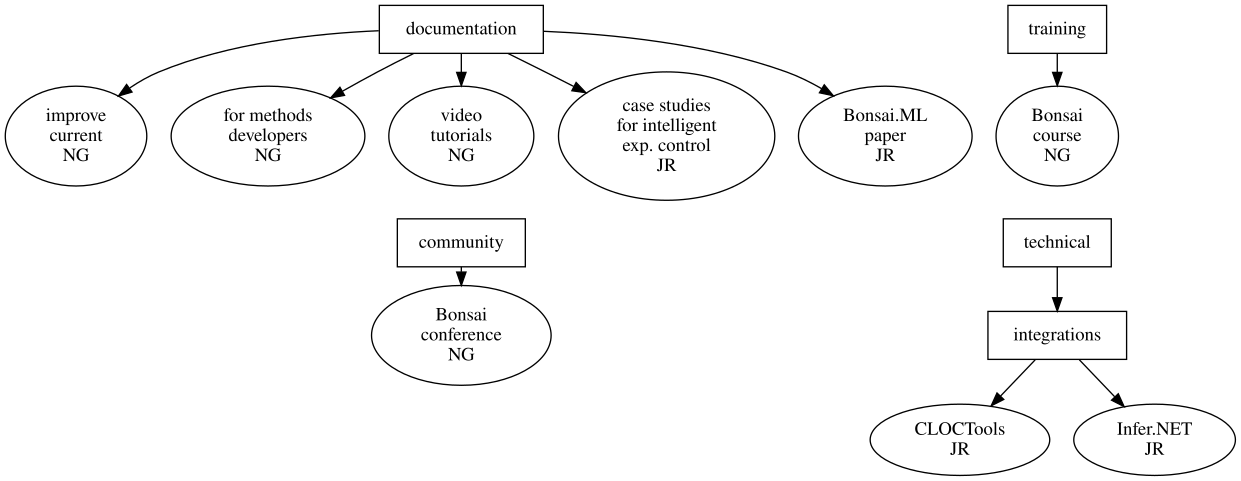
\includegraphics[width=6in]{activitiesGraphs/activities_larger.png}

    \caption{Proposed activities. The initials below each task name indicate
    the responsible team member (JR: Joaquin Rapela, NG: NeuroGEARS Ltd). See
    text for details.}

\end{figure}

\subsection*{Approach}

\subsubsection*{Documentation}

Background: The Bonsai.ML project has maintained a strong commitment to producing high-quality documentation to support both experimental neuroscience users and machine learning method developers. The documentation of the current Bonsai.ML project includes a few articles introducing the packages with installation guides for each package, an automatically generated API reference for the C\# codebase, and some examples demonstrating various use cases. Currently, there is no documentation for the Python code integrated into the packages, nor are there any video tutorials or developer-focused documentation.

Our team has been approached by several users of the package who have expressed concerns about the current state of the documentation, particularly regarding the documentation structure. There is redundancy in places in the documentation and a lack of clarity in others. For instance, the installation instructions for Bonsai.ML.LinearDynamicalSystems is included in the "Getting Started" section of the Linear Dynamical Systems examples. Additionally, these instructions are very similar to those found in other Bonsai.ML - Python based packages, leading to additional redundancy. Conversely, the current documentation lacks critical statistical information in several parts, including packages implementing specific machine learning models, and examples (both with simulated data and real-world data). This lack of clarity and redundancy has made it difficult for users to find the information they need, leading to unnecessary user-friction driving new users away from the project.

Furthermore, the current documentation does not adequately address the needs of machine learning method developers. Our team has documented several approaches for integrating machine learning models into Bonsai, but this information is currently distributed across various sources, including GitHub repos, discussion issues, pull requests, and examples. Our project lacks a dedicated, centralized resource that provides comprehensive documentation for method developers looking to create new machine learning functionality in Bonsai using the approaches our team has developed.

To address these issues, we have identified several key areas of improvement that we believe will enhance the usability and accessibility of the documentation for both user groups. These include:

* Restructure and expand the existing documentation to match the style of established machine learning libraries. For this, our team will base our documentation style on the popular scikit-learn documentation. We will add to Bonsai.ML's documentation by creating dedicated sections for installation, user guides, detailed statistical explanations of methods, API reference, examples, and troubleshooting.
* Provide additional tailored, comprehensive examples and user guides to demonstrate applications of Bonsai.ML methods for both neuroscientists and machine learning developers.
* Produce video tutorials to complement written documentation, catering to different learning styles and improving accessibility.
* Enhance developer-focused documentation, including detailed guides and tutorials for method developers on how to create and integrate new machine learning methods into Bonsai using 3 different approaches: Python, C\# scripting, and TorchSharp.


\paragraph{Tasks:}\mbox{}\\

\begin{description}

    \item[doc\_review:] Conduct a thorough review of the existing documentation (Python, C\#, and TorchSharp). Identify redundancies, outdated content, missing sections compared to scikit-learn package.

    \item[style\_guide:] Create a Bonsai.ML style guide which will include conventions for: documentation, code formatting, naming, and video tutorial format. These will draw on inspirations from the style guides and best practices put forth by \href{https://learn.microsoft.com/en-us/dotnet/csharp/fundamentals/coding-style/coding-conventions}{Microsoft}, the \href{https://github.com/dotnet/runtime/blob/main/docs/coding-guidelines/coding-style.md}{dotnet community}, and the developers of \href{https://github.com/pytorch/pytorch/blob/main/CONTRIBUTING.md}{PyTorch}.
    
    \item[examples\_improvement:] Improve the existing examples by restructuring them to match the new style guide. Each example will include a detailed explanation of the Bonsai workflow, the mathematical/statistical basis of the model, and clarifications on assumptions and data requirements.

    \item[examples\_new:] Develop at least 3 new examples that showcase complete applications of Bonsai.ML. These examples will cover: neural signal processing, real-time latent visualization, and clustering of behavioural data. Each example will have detailed workflow descriptions, information on the models and assumptions, and explanations of the datasets.

    \item[user\_guides:] Write new, comprehensive user guides to teach users about key ML concepts and how to use the Bonsai.ML libraries correctly. User guides will come in 2 flavours: one will be geared towards neuroscientists who may have familiarity with conducting experiments but are less familiar with ML techniques. These will focus more on teaching core concepts of math, statistics, and machine learning. The other style will be geared more towards ML developers and will focus more on reactive, online data streams and approaches for integrating ML models into Bonsai. These user guides will include how to create a new Bonsai.ML package with Python, C\# and expression scripting, and integrating models via TorchSharp and other native C\# libraries.
    
    \item[troubleshooting:] Create a troubleshooting section to address common issues users may encounter when using Bonsai.ML packages. This section will include solutions to frequently asked questions, common errors, and tips for debugging.
    
    \item[video\_series:] Produce at least 3 video tutorials and demos, hosted on YouTube, and embed them directly into the documentation. These videos will cover key topics such as installation, user guides, and examples. The 3 videos will be: 1) Installation and getting started with Bonsai.ML, 2) Integrating custom models into Bonsai using Python, C\#, and TorchSharp, and 3) Building a Bonsai.ML application to perform closed-loop stimulation using online neural signal processing.

\end{description}

\paragraph{Impact:}
Improving the documentation of Bonsai.ML will directly improve the code's maintainability, reduce technical debt for maintainers and contributors, and expand the project's reach. The expansion of the documentation will also greatly enhance usability of Bonsai.ML for two core communities: experimental neuroscientists and machine learning developers. Clearer, better-structured resources aimed at these groups will reduce barriers to usage and onboarding friction. Specifically, we will provide experimental neuroscientists with the knowledge to adopt and implement powerful ML tools for real-time experimental applications. Additionally, we will provide ML developers interested in integrating their models into Bonsai with the guidance from experienced, Bonsai.ML developers, to extend ML functionality in Bonsai. By adding examples, comprehensive user guides, troubleshooting resources, and video tutorials, we will create robust, easy-to-navigate documentation, modeled after leading ML libraries, that will greatly boost Bonsai.ML's maintenance and adoption. Ultimately, these improvements will lower duplication of effort, standardize best practices, broaden Bonsai.ML's reach, and ensure long-term sustainability through a stronger and more engaged user and developer community.

\paragraph{Milestones and Indicators:}\mbox{}\\

\begin{description}

    \item[doc\_m1]: Documentation review completed.
    \item[doc\_i1]: Publically shared document on GitHub detailing restructuring plan. The plan will include both pitfalls of the current documentation and proposed changes for the new documentation.
    
    \item[doc\_m2]: Bonsai.ML style guide finalized and merged into the repository.
    \item[doc\_i2]: Publically shared document avaiable at docs/contributing.md on GitHub. This will include information on coding style, contributing code/PRs, documentation, unit testing, and naming conventions.
    
    \item[doc\_m3]: All existing examples reviewed and updated to conform to the style guide.
    \item[doc\_i3]: All existing examples updated with new documentation to address missing information on mathematical/statistical background, data assumptions, and Bonsai workflows.
    
    \item[doc\_m4]: Three new examples published (neural signal processing, real-time latent visualization, behavioural clustering).
    \item[doc\_i4]: Each new example will be documented with explanation of the workflow components, mathematical basis of models/algorithms, and assumptions about the data.
    
    \item[doc\_m5]: New user guides published for both neuroscientists and ML developers.
    \item[doc\_i5]: At least 2 guides (2 per audience type) completed.
    
    \item[doc\_m6]: Troubleshooting section added to documentation website.
    \item[doc\_i6]: Section will include at least 10 common issues/errors addressed.
    
    \item[doc\_m7]: Video tutorials produced, uploaded to YouTube, and embedded in documentation.
    \item[doc\_i7]: Video 1: "Installation and Getting Started with Bonsai.ML" - posted by April. Video 2: "Integrating Custom Models with Python, C#, and TorchSharp" - posted by May. Video 3: "Building a Closed-Loop Experiment with Bonsai.ML." - posted by September. Video engagement will be monitored by tracking views, likes, and comments.

\end{description}

\noindent\rule{\textwidth}{1pt}
\subsubsection*{Training}

\paragraph{Summary:} Organise Bonsai course, with a Bonsai.ML module.

\paragraph{Previous work:} Since 2017, NeuroGEARS Ltd has organised at least
two Bonsai courses per year at different universities, and
\href{https://bonsai-rx.org/learn/}{some of them} can be viewed online. We will
deliver a one-week-long Bonsai course, hosted at the Sainsbury Wellcome Centre,
for approximately 20 students, targeted to Bonsai users with intermediate
understanding of the language. The structure of the course will be similar to
previous ones (e.g., \href{https://neurogears.org/st-andrews-2024/}{2024 Bonsai
Course at St.~Andrews University}).

\paragraph{Outputs:} course delivery, online course material (including lecture
slides, worksheets and video recordings).

\paragraph{Responsible team members:} GL, JR.

\noindent\rule{\textwidth}{1pt}
\subsubsection*{Collaborations}

\paragraph{Collaboration 1: forecasting animal behaviour for zero-lag stimulus
presentation in augmented-reality experiments.} Prof.~Aman Saleem,
\href{https://www.saleemlab.com/}{Saleem Lab}, Institute of Behavioural
Neuroscience, University College London, UK.


\begin{description}

    \item[Background:] In augmented reality experiments, particularly in
        neuroscience, precise stimulus timing is critical, yet unavoidable
        system delays mean that visual stimuli often appear slightly later than
        intended. This latency is especially problematic when linking neural
        activity to sensory input or behaviour. To address this, we will use
        algorithms that forecast animal position and head orientation, allowing
        stimuli to be pre-rendered and displayed in synchrony with the
        subject's actual position and head orientation.

    \item[Previous work:] In the 2024 Bonsai conference we began conversations
        with Prof.~Saleem about using predictive algorithms, like state-space
        models, to improve augmented reality experiments in animals. We
        implemented in Python a
        \href{https://github.com/joacorapela/collaborationAman/blob/master/reports/ekfForKinematicsAndHeadOrientation/ekfForKinematicsAndHeadOrientation.pdf}{
            nonlinear state-space model, and the extended Kalman filter
            algorithm} to estimate the model parameters, in order to forecast,
        using video recordings, position and head orientation of mice exploring
        a circular arena surrounded by a 360 degree visual display screen. We identified
        experimental and methodological improvements for the next iteration of
        the collaboration.

    \item[Future work:] We will further test the accuracy of the previous model
        and estimation algorithm and, if needed, explore alternatives. For this
        we will use artificially generated data with ground truth. The Saleem
        laboratory will improve experimental procedures. Then we will evaluate
        the performance of the Bonsai.ML forecaster in new animal behavioural
        data.

    \item[Outcomes:] We will document the activities of the collaboration, create a new
        Bonsai.ML forecasting package, and publish the outcomes of the
        collaboration in a scientific journal.

    \item[Responsible team member:] JR.

\end{description}

\paragraph{Collaboration 2: estimating latent variables for high-channel-count
Neuropixels recordings, in real time, while recordings are being performed.}
Dr.~Josh Siegle, head of the electrophysiology group, Allen Institute for
Neural Dynamics, US.

\begin{description}

    \item[Background:] Visualisation is central to scientific inquiry,
        especially in neuroscience. Yet, modern high-density recordings from
        hundreds or thousands of electrodes pose major challenges for clear,
        real-time visualisation. At the Gatsby Unit, we pioneered single-trial
        dimensionality reduction with latent-variable models \citep{yuEtAl09},
        and extended these approaches in later work, e.g.
        \citep{dunckerAndSahani18}, supported by open-source software
        (\href{https://github.com/joacorapela/svGPFA}{svGPFA}). However, all
        current latent-variable methods operate offline, after data collection.
        In this project we will integrate a state-space model into Bonsai.ML to
        estimate and visualise latent variables online, during
        high-channel-count recordings.

    \item[Previous work:] We have developed a
        \href{https://joacorapela.github.io/ssm/auto_examples/neuralLatents/plot_MC_MAZE_SMALL.html#sphx-glr-auto-examples-neurallatents-plot-mc-maze-small-py}{linear-dynamical-systems
        model and estimation methods to infer latent variables in real time
        from high-channel-count electrophysiological recording}, and we are now
        integrating it into Bonsai.ML.


    \item[Future work:] Evaluate the real-time performance of the Bonsai.ML
        latents estimation method with previously recorded data replayed in
        real time, and later with live neural recordings collected by the group
        of Dr.~Siegle at the AIND.

    \item[Outcomes:] Bonsai.ML neural latent package, documented with examples
        from this collaboration. Paper reporting scientific findings, and
        real-time performance metrics, of the Bonsai.ML neural latents package
        applied to neural recordings from the AIND.

    \item[Responsible team member:] JR.

\end{description}

\noindent\rule{\textwidth}{1pt}
\subsubsection*{Integrations}

\subsubsection*{Probabilistic programming: Infer.NET}

\paragraph{Background:} Most of the probabilistic models currently integrated
into Bonsai are implemented in Python. These serve as excellent demonstrations
of how Python applications can connect to the Bonsai ecosystem, and they are
central to our aim of attracting Python developers to contribute to Bonsai.ML.

However, Python implementations are substantially slower than equivalent C\#
code. For demanding real-time applications, C\# implementations are preferable,
especially when expressed in a probabilistic programming language (PPL).

The existing Python and C\# implementations of probabilistic models (e.g.,
linear dynamical systems, hidden Markov models, Bayesian linear regression —
see
\href{https://bonsai-rx.org/machinelearning/examples/README.html}{examples})
are relatively complex and heterogeneous, making them harder to maintain. In
contrast, implementations in a C\# PPL would be faster, simpler, and more
homogeneous, reducing errors and improving maintainability.

Fortunately, C\# has an excellent PPL:
\href{https://dotnet.github.io/infer/}{Infer.NET}, developed at Microsoft
Research Cambridge since 2004, used in
\href{https://dotnet.github.io/infer/papers.html}{hundreds of papers}, and
\href{https://www.microsoft.com/en-us/research/blog/the-microsoft-infer-net-machine-learning-framework-goes-open-source/}{open-sourced
in 2018}.  Infer.NET uses deterministic approximate inference, enabling fast
and scalable solutions. For
\href{https://www.microsoft.com/en-us/research/blog/the-microsoft-infer-net-machine-learning-framework-goes-open-source/}{example},
it has powered systems that extract knowledge from billions of web pages
(petabyte-scale data) — the kind of scalability critical for real-time
inference in Bonsai.

Message passing is a natural connection point between Bonsai and Infer.NET.
Infer.NET uses message passing for approximate inference, while Bonsai relies
on message passing for reactive computations. Exposing Infer.NET’s message
passing algorithms as Bonsai nodes will allow users to seamlessly combine
efficient inference with reactive experimental control.

We will re-implement in Infer.NET all the probabilistic models previously
integrated into Bonsai using Python or C\#. This integration will accelerate
inference, simplify and standardise inference programs, and empower Bonsai
users to create new probabilistic models and inference algorithms with just a
few lines of code. By making powerful yet easy-to-use inference methods
accessible to experimental neuroscientists, this project has the potential to
profoundly advance scientific discovery.

\paragraph{Previous work:} Our Microsoft collaborator, Dr.~Tom Minka, invented
a seminal algorithm for inference in graphical models, the Expectation
Propagation algorithm~\citep{minka01}, and is the lead developer of Infer.NET.
Please refer to his letter of support.

\paragraph{Responsible team member:} JR.

\paragraph{Outputs:}\mbox{}\\

\begin{itemize}

    \item Bonsai nodes implementing Infer.NET inference methods
    \item online Bayesian linear regression implemented in Bonsai.ML--Infer.NET
    \item linear dynamical systems implemented in Bonsai.ML--Infer.NET
    \item hidden Markov model implemented in Bonsai.ML--Infer.NET
    \item point-process decoder implemented in Bonsai.ML--Infer.NET
    \item documentation, tutorials and use cases on how to work with
probabilistic programming models in Bonsai--Infer.NET \end{itemize}

\subsubsection*{Closed-loop optogenetic control tools: CLOCTools}

\paragraph{Background:} Closed-loop neural control represents a transformative
advance in neuroscience:  rather than delivering stimulation at fixed,
open-loop schedules, it enables precisely timed interventions based on ongoing
brain and behavioural activity. This paradigm allows researchers to move beyond
observing correlations to  directly testing causal mechanisms of neural
dynamics, plasticity, and behaviour. Critically, closed-loop stimulation has
already proved transformative in the  clinic, for example in deep brain
stimulation for Parkinson’s disease and  epilepsy, while its extension to other
disorders (e.g. depression, obsessive  compulsive disorder) remains an active
area of research. Despite this promise, widespread adoption has been limited
by the lack of accessible, well-engineered,  and sustainable software
frameworks for real-time experimental control.

Prof.~Garrett Stanley (Georgia Tech and Emory University, US) is a pioneer in
closed-loop neuroscience, having developed groundbreaking methods that combine
real-time neural control with systems neuroscience. He recently contacted us to
explore integrating their existing
\href{https://cloctools.github.io/}{CLOCTools}, originally implemented in
RTXI/C++, into Bonsai.ML.  This represents a unique opportunity: Bonsai already
excels at real-time closed-loop control in behavioural experiments, and
extending it to include state-of-the-art closed-loop neural control will
position the platform as the first sustainable, general-purpose framework for
both levels of experimentation.

An important reason for the poor uptake of closed-loop methods in neuroscience
could be that existing implementations are often ad hoc, difficult to install
or  extend, and not integrated with software for experimental control. By
providing Bonsai users with accessible, open-source, and sustainably engineered
tools for closed-loop control, we will directly address this barrier and enable
a new type of experimentation where researchers can both read and write the
neural code in real time. This will accelerate discovery across both basic and
translational neuroscience.

\paragraph{Previous work:} Members of Prof.~Stanley’s lab have already
prototyped some of their closed-loop control methods in Bonsai using our
\href{https://bonsai-rx.org/python-scripting/}{Python scripting interface}.
Please refer to the repositories in the
\href{https://github.com/ndac-bonsai}{ndcac-bonsai} organisation containing
these prototypes (ndac stands for neural dynamic adaptive control).

\paragraph{Responsible team members:} JR

\paragraph{Subtasks:}\mbox{}\\

\begin{itemize}

    \item implement in C\# the functionality in the repositories of the
        organization \href{https://github.com/ndac-bonsai}{ndac-bonsai}.

    \item deploy a comprehensive battery of test cases to check the correctness
        of the C\#/Bonsai implementation against the Python one.

    \item extend functionality of Bonsai development environment to allow users
        graphically build probabilistic models.

    \item develop documentation, tutorials and use cases for experimental
        neuroscientists with no training on optimal feedback control.

\end{itemize}

\noindent\rule{\textwidth}{1pt}
\subsubsection*{Governance}

We will create a Bonsai.ML steering committee that will provide us strategic
oversight on this project and advise us on building a long-term development
roadmap for Bonsai.ML.

Several renowned experimental and computational neuroscientists around the
world are heavily invested in Bonsai, are very interested in adding ML
functionality to their Bonsai workflows and have agreed to join the Bonsai.ML
steering committee. We list them below.

\begin{description}

    \item[Prof.~Thomas Mrsic-Flogel,] director of the SWC, project lead on the
        BBSRC grant that funded the creation of Bonsai.ML, and project lead on
        this proposal. Bonsai is the main software for experimental control at
        the SWC.

    \item[Prof.~Maneesh Sahani,] director of the GCNU, project co-lead on the
        BBSRC grant that funded the creation of Bonsai.ML, and project co-lead
        on this proposal.

    \item[Prof.~Garrett Stanley,] leader of the Laboratory for the Control of
        Neural Systems, Georgia Tech, US. Expert on close-loop control of
        neurophysiological systems. He contacted us to migrate to Bonsai
        a package for real-time cortical state estimation and the CLOCTools
        referred above, both originally written in C++/RTXI.

    \item[Prof.~Aman Saleem,] director of the Saleem Lab at the Institute for
        Behavioural Neuroscience, University College London. Prof.~Saleem is the
        author of \href{https://bonvision.github.io/}{Bon-Vision}, a software
        package that creates and controls visual environments in close loop,
        built on top of Bonsai.

    \item[Prof.~Josh Siegle,] senior scientist and lead of the
        electrophysiology group at the Allen Institute for Neural Dynamics,
        where Bonsai is the only software for experimental control.

    \item[Prof.~Ken Harris,] co-director of the Cortexlab, University College
        London, and founding director of the International Brain Laboratory,
        that uses Bonsai for reproducible experimental control across 22
        laboratories around the world.

    \item[Prof.~Athena Akrami,] director of the Learning, Inference and Memory
        Lab, at the SWC, that uses Bonsai for experimental control.

\end{description}

\noindent\rule{\textwidth}{1pt}
\subsection*{Management}

We will conduct management activities at different frequencies:

\begin{description}

    \item[Twice a year:] we will generate a progress report, which will be
        publicly available, and hold meetings with the steering committee to
        discuss it and receive expert advise. Minutes from these meeting will
        be published openly to maintain transparency.

    \item[Every three months:] we will hold meetings between the project lead, TMF, the
        project co-lead, MS, the RSE, JR, and
        the external project co-lead, GL, to evaluate the project progress.

    \item[Weekly:] as has been our practice since the start of the Bonsai.ML
        project, the junior and senior RSEs will meet with the external project
        co-lead to discuss issues that appeared during the week, review
        activities for the following week, and adjust project directions.

    \item[Daily:] the offices of the senior and junior RSEs are next to each
        other, enabling discussions to manage spontaneous project issues.

\end{description}

Meetings with collaborators will be arranged as needed.
%
At the SWC, GCNU and NG we are experimental and computational neuroscientists
with successful collaborative experience, and we have no doubt that the
proposed collaborations will be of the same kind,
%
specially since we have successfully interacted in the past with most of the
propose collaborators.
%
Please refer to their letters of support.
